\documentclass[border=10pt]{standalone}
\usepackage{tikz}
\usepackage{xcolor}
\usetikzlibrary{shapes.geometric, positioning}

\definecolor{entityblue}{RGB}{173, 216, 230} % light blue

\begin{document}
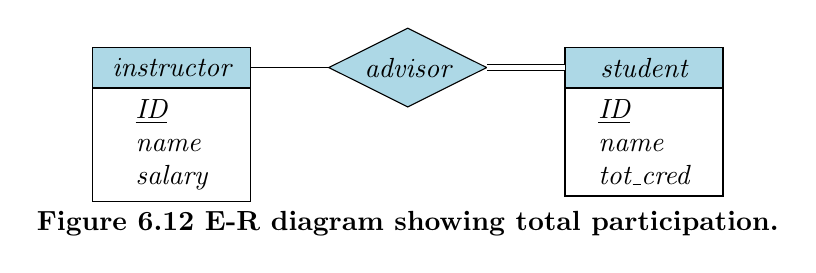
\begin{tikzpicture}[
  font=\itshape,
  entityheader/.style={
    draw=black,
    fill=entityblue,
    minimum width=2cm,
    minimum height=0.5cm,
    align=center,
  },
  entitybody/.style={
    draw=black,
    fill=white,
    minimum width=2cm,
    minimum height=1cm,
    align=left,
    inner xsep=6pt,
    inner ysep=4pt,
  },
  relationship/.style={
    draw=black,
    fill=entityblue,
    diamond,
    aspect=2,
    minimum width=1.4cm,
    minimum height=0.9cm,
    align=center,
    inner sep=2pt,
  }
]

  % === FIGURE 6.12: Total participation ===
  % INSTRUCTOR (left)
  \node[entityheader] (i-h) at (0, 2) {\normalsize instructor};
  \node[entitybody, below=0pt of i-h] (i-b) {\underline{ID}\\ name\\ salary};
  \draw (i-h.south west) -- (i-h.south east);
  \draw (i-h.north west) rectangle (i-b.south east);

  % STUDENT (right)
  \node[entityheader] (s-h) at (6, 2) {\normalsize student};
  \node[entitybody, below=0pt of s-h] (s-b) {\underline{ID}\\ name\\ tot\_cred};
  \draw (s-h.south west) -- (s-h.south east);
  \draw (s-h.north west) rectangle (s-b.south east);

  % ADVISOR (diamond, center)
  \node[relationship] (adv) at (3, 2) {\normalsize advisor};

  % Lines: single instructor--advisor, DOUBLE student--advisor (total participation)
  \draw (i-h.east) -- (adv.west);
  \draw[double, double distance=1.5pt] (s-h.west) -- (adv.east);

  % Caption
  \node[font=\normalfont\bfseries, anchor=north] at (3, 0.3) {Figure 6.12 E-R diagram showing total participation.};

\end{tikzpicture}

\vspace{1.5cm}

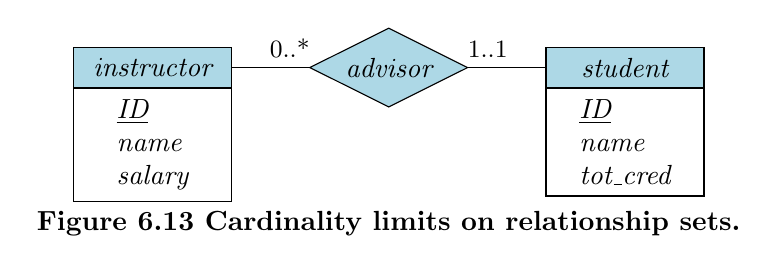
\begin{tikzpicture}[
  font=\itshape,
  entityheader/.style={
    draw=black,
    fill=entityblue,
    minimum width=2cm,
    minimum height=0.5cm,
    align=center,
  },
  entitybody/.style={
    draw=black,
    fill=white,
    minimum width=2cm,
    minimum height=1cm,
    align=left,
    inner xsep=6pt,
    inner ysep=4pt,
  },
  relationship/.style={
    draw=black,
    fill=entityblue,
    diamond,
    aspect=2,
    minimum width=1.4cm,
    minimum height=0.9cm,
    align=center,
    inner sep=2pt,
  }
]

  % === FIGURE 6.13: Cardinality limits ===
  % INSTRUCTOR (left)
  \node[entityheader] (i-h) at (0, 2) {\normalsize instructor};
  \node[entitybody, below=0pt of i-h] (i-b) {\underline{ID}\\ name\\ salary};
  \draw (i-h.south west) -- (i-h.south east);
  \draw (i-h.north west) rectangle (i-b.south east);

  % STUDENT (right)
  \node[entityheader] (s-h) at (6, 2) {\normalsize student};
  \node[entitybody, below=0pt of s-h] (s-b) {\underline{ID}\\ name\\ tot\_cred};
  \draw (s-h.south west) -- (s-h.south east);
  \draw (s-h.north west) rectangle (s-b.south east);

  % ADVISOR (diamond, center)
  \node[relationship] (adv) at (3, 2) {\normalsize advisor};

  % Lines with cardinality labels (near the diamond)
  \draw (i-h.east) -- (adv.west) node[pos=0.75, above, font=\normalfont\small] {0..*};
  \draw (s-h.west) -- (adv.east) node[pos=0.75, above, font=\normalfont\small] {1..1};

  % Caption
  \node[font=\normalfont\bfseries, anchor=north] at (3, 0.3) {Figure 6.13 Cardinality limits on relationship sets.};

\end{tikzpicture}
\end{document}
